%\iffalse
\let\negmedspace\undefined
\let\negthickspace\undefined
\documentclass[journal,12pt,twocolumn]{IEEEtran}
\usepackage{cite}
\usepackage{amsmath,amssymb,amsfonts,amsthm}
\usepackage{algorithmic}
\usepackage{graphicx}
\usepackage{textcomp}
\usepackage{xcolor}
\usepackage{txfonts}
\usepackage{listings}
\usepackage{enumitem}
\usepackage{mathtools}
\usepackage{gensymb}
\usepackage{comment}
\usepackage[breaklinks=true]{hyperref}
\usepackage{tkz-euclide} 
\usepackage{listings}
\usepackage{gvv}                                        
\def\inputGnumericTable{}                                 
\usepackage[latin1]{inputenc}                                
\usepackage{color}                                            
\usepackage{array}                                            
\usepackage{longtable}                                       
\usepackage{calc}                                             
\usepackage{multirow}                                         
\usepackage{hhline}                                           
\usepackage{ifthen}                                           
\usepackage{lscape}

\newtheorem{theorem}{Theorem}[section]
\newtheorem{problem}{Problem}
\newtheorem{proposition}{Proposition}[section]
\newtheorem{lemma}{Lemma}[section]
\newtheorem{corollary}[theorem]{Corollary}
\newtheorem{example}{Example}[section]
\newtheorem{definition}[problem]{Definition}
\newcommand{\BEQA}{\begin{eqnarray}}
 \newcommand{\EEQA}{\end{eqnarray}}
\newcommand{\define}{\stackrel{\triangle}{=}}
\theoremstyle{remark}
\newtheorem{rem}{Remark}
\begin{document}
 \bibliographystyle{IEEEtran}
 \vspace{3cm}
 \title{\textbf{XE 71}}
 \author{EE23BTECH11048-Ponugumati Venkata Chanakya$^{*}$% <-this % stops a space
 }
 \maketitle
 \newpage
 \bigskip
 \renewcommand{\thefigure}{\theenumi}
 \renewcommand{\thetable}{\theenumi}
 \textbf{QUESTION:}
 A spring mass system is shown in the figure . Take the value of acceleration  due to gravity as $g=9.81m/s^2$.The static deflection due to weight and the time period of the oscillations,respectively,are\\
 \begin{figure}[h!]
    \centering
    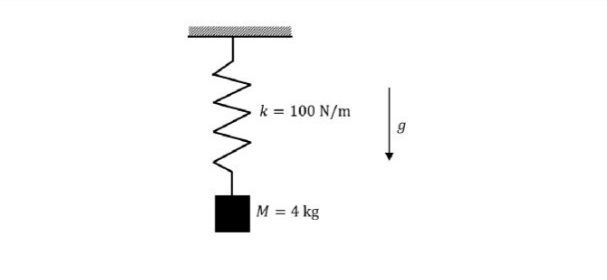
\includegraphics[width=0.4\textwidth]{figs/fig1.jpg}
    \caption{ }
    \label{fig}
\end{figure}

\solution
\begin{enumerate}
    \item Static deflection due to weight(sdw)\\
    let x be sdw.\\
    At mean position in equilibrium\\
    \begin{align}
        Mg&=kx\\
        4\cdot9.81&=100x\\
        39.24&=100x\\
        x&=0.3924m\\
        x&=39.24cm
    \end{align}
     \item Time period of oscilattion\\
     \begin{align}
           F&=-kx^2\\
           ma&=-kx^2\\
           m(-\omega^2 x^2)&=-kx^2\\
           \omega &= \sqrt{\frac{k}{m}}\\
           \omega&=\sqrt{\frac{100}{4}}\\
           \omega&=5\\
           T&=\frac{2\pi}{\omega}\\
           T&=\frac{2\pi}{5}seconds
     \end{align}
    The static deflection due to weight and the time period of the oscillations,respectively,are $39.24cm and \frac{2\pi}{5}seconds$
\end{enumerate}

\end{document}

